\documentclass[12pt]{report}

\usepackage{amssymb, fullpage, amsmath, esint}
\usepackage{graphicx}

\newtheorem{problem}{Problem}

\newenvironment{solution}[1][\it{Solution}]{\textbf{#1. } }{$\square$}

\graphicspath{ {./} }

\allowdisplaybreaks

\pagestyle{empty}

\def\Z{{\mathbb Z}}
\def\Q{{\mathbb Q}}
\def\C{{\mathbb C}}
\def\R{{\mathbb R}}
\def\N{{\mathbb N}}
\def\eps{{\epsilon}}
\def\O{{\mathcal{O}}}
\newcommand{\floor}[1]{{\left\lfloor#1\right\rfloor}} % Floor function
\newcommand{\ceil}[1]{{\left\lceil#1\right\rceil}} % Ceiling function
\newcommand{\paren}[1]{{\left(#1\right)}} % Parentheses ()
\newcommand{\brac}[1]{{\left\{#1\right\}}} % Curly braces {}
\newcommand{\braces}[1]{{\left[#1\right]}} % Braces []
\newcommand{\abrac}[1]{{\left\langle#1\right\rangle}} % Angle Braces <>
\newcommand{\abs}[1]{{\left|#1\right|}} % Absolute value
\newcommand{\norm}[1]{{\left\|#1\right\|}} % Norm
\newcommand{\eval}[2]{\right|_{#1}^{#2}} % Evaluate

\newcommand{\pp}[2]{\frac{\partial #1}{\partial #2}} % Partial of 1 wrt 2
\newcommand{\ppn}[3]{\frac{\partial^{#1} #2}{\partial #3^{#1}}} % nth Partial of 1 wrt 2
\newcommand{\dd}[2]{\frac{\mathrm{d} #1}{\mathrm{d} #2}} % Partial of 1 wrt 2
\newcommand{\ddn}[3]{\frac{\mathrm{d}^{#1} #2}{\mathrm{d} #3^{#1}}} % nth Partial of 1 wrt 2

\def\ointcc{{\ointctrclockwise}} %counter clockwise contour integral
\def\ointc{{\ointclockwise}} %clockwise contour integral

%dash integral 
\def\Xint#1{\mathchoice
   {\XXint\displaystyle\textstyle{#1}}%
   {\XXint\textstyle\scriptstyle{#1}}%
   {\XXint\scriptstyle\scriptscriptstyle{#1}}%
   {\XXint\scriptscriptstyle\scriptscriptstyle{#1}}%
   \!\int}
\def\XXint#1#2#3{{\setbox0=\hbox{$#1{#2#3}{\int}$}
     \vcenter{\hbox{$#2#3$}}\kern-.5\wd0}}
\def\ddashint{\Xint=}
\def\dashint{\Xint-}


\begin{document}

\large

\begin{center}
 Math 573 Homework 4\\
 Due Soon\\
 By Marvyn Bailly\\
\end{center}

\normalsize

\hrule

%---------------%
%---Problem 1---%
%---------------%

%--Part C NEED TO TYPE--$

\begin{problem}
    Consider the Modified Vector Derivative NLS equation
$$
B_t+(\|B\|^2B)_x+\gamma (e_1\times
B_0)\left(e_1\cdot (B_x\times
B_0)\right)+e_1\times B_{xx}=0.
$$
This equation describes the transverse
propagation of nonlinear Alfv\'en waves in
magnetized plasmas. Here $B=(0,u,v)$, $e_1=(1,0,0)$,
$B_0=(0,B_0,0)$, and $\gamma$ is a constant. The boundary conditions are
$B\rightarrow B_0$, $B_x \rightarrow 0$ as $|x|\rightarrow
\infty$.
By looking for stationary solutions $B=B(x-W t)$, one obtains a
system of ordinary differential equations. Integrating once, one obtains a
first-order system of differential equations for $u$ and $v$.
\begin{itemize}
\item[a)] Show that this system is
Hamiltonian with canonical Poisson structure, by constructing its Hamiltonian
$H(u,v)$.
\item[b)]
Find the value of the Hamiltonian such that the boundary conditions are
satisfied. Then $H(u,v)$ equated to this constant value defines a curve in the
$(u,v)$-plane on which the solution lives. In the equation of this curve, let
$U=u/B_0$, $V=v/B_0$, and $W_0=W/B_0^2$. Now there are only two parameters in the
equation of the curve: $W_0$ and $\gamma$.
\item[c)] With $\gamma=1/10$, plot the curve for $W_0=3$, $W_0=2$, $W_0=1.1$,
$W_0=1$, $W_0=0.95$, $W_0=0.9$. All of these curves have a singular point at
$(1,0)$. This point is an equilibrium point for the Hamiltonian system,
corresponding to the constant solution which satisfies the boundary condition.
The curves beginning and ending at this equilibrium point correspond to
soliton solutions of the Modified Vector Derivative  NLS equation. How many soliton
solutions are there for the different velocity values you considered? Draw a
qualitatively correct picture of the solitons for all these cases.
\end{itemize}
\end{problem}

\begin{solution}
    (Worked with Kaitlynn throughout homework and Cade on number 8)

    \noindent
    Consider the Modified Vector Derivative NLS equation
    \[ 
        B_t+(\|B\|^2B)_x+\gamma (e_1\times B_0)\left(e_1\cdot (B_x\times B_0)\right)+e_1\times B_{xx}=0,
    \]
    where $B = (0,u,v)^T$, $e_1 = (1,0,0)^T$, $B_0 = (0, B_0, 0)^T$ and $\gamma$ is a constant with boundary conditions $B \to B_0, B_x \to 0$ as $|x| \to \infty$. 
    
    \begin{enumerate}
        \item [a)]
        To reduce the system to a first-order system, consider when $B = B(x-Wt)$. Then the partials are given by
        \begin{align*}
            B_t &= -WB_z(x - Wt)\\
            B_x &= B_z(x - Wt)\\
            B_{xx} &= B_{zz}(x - Wt).
        \end{align*}
        Plugging these into the NLS equation we get
        \begin{align*}
            0 &= B_t + (u^2B + v^2B)_z + \gamma(e_1 \times B_0)(e_1 \cdot (B_x \times B_0)) + e_1 \times B_x\\
            &=\begin{pmatrix}
                0\\u_t\\v_t
            \end{pmatrix} + \pp{}{x}\begin{pmatrix}
                0\\u^3 + v^2 u\\vu^2+v^3
            \end{pmatrix} + \begin{pmatrix}
                0\\0\\\gamma B_0
            \end{pmatrix}\paren{\begin{pmatrix}
                1\\0\\0
            \end{pmatrix}\begin{pmatrix}
                -v_xB_0\\0
            \end{pmatrix}} + \begin{pmatrix}
                0\\-v_{xx}\\u_{xx}\\
            \end{pmatrix}\\
            &= \begin{pmatrix}
                0\\u_t\\v_t
            \end{pmatrix} + \pp{}{x}\begin{pmatrix}
                0\\u^3 + v^2 u\\vu^2+v^3
            \end{pmatrix} + \begin{pmatrix}
                0\\0\\-v_xB_0^2\gamma
            \end{pmatrix} + \begin{pmatrix}
                0\\-v_{xx}\\u_{xx}\\
            \end{pmatrix}.
        \end{align*}
        Splitting this into two equations and using the partials we computed we get
        \[ 
            \begin{cases}
                -Wu_z + (u^3 + v^2u)_z - v_{zz} = 0\\
                -Wv_z + (vu^2 + v^3)_z - \gamma B_0^2v_z + u_{zz} = 0
            \end{cases},
        \]
        and integrating both sides with respect to $z$ gives
        \[ 
            \begin{cases}
                -Wu + (u^3 + v^2u) - v_{z} = \alpha\\
                -Wv + (vu^2 + v^3) - \gamma B_0^2v + u_{z} = \beta
            \end{cases},
        \]
        where $\alpha$ and $\beta$ are integration constants. From our boundary conditions we have that $u \to B_0$, $v \to 0$, $u_z \to 0$ and $v_z \to 0$ as $|x| \to \infty$. Thus $\beta = 0$ and $\alpha = -W \beta_0 + \beta^3$. Since this is an ODE, let
        \[ 
            u_{z} = \pp{\mathcal{H}}{v} ~~~ v_{z} = -\pp{\mathcal{H}}{u}
        \]
        Then our system becomes
        \[ 
            \begin{cases}
                -Wu + (u^3 + v^2u) + W \beta_0 - \beta^3 = v_{z} = -\pp{\mathcal{H}}{u}\\
                Wv - vu^2 - v^3 + \gamma B_0^2v = u_{z} = \pp{\mathcal{H}}{v}
            \end{cases}.
        \]
        Integrating both sides gives
        \[ 
            \mathcal{H} = \frac{W}{2}U^2 - \frac{1}{4}u^4 - \frac{v^2}{2}u^2 - WB_0u + B_0^3u + A(v),
        \]
        and 
        \[ 
            \mathcal{H} = \frac{W}{2}v^2 - \frac{u^2}{2}v^2 - \frac{1}{4}v^4 + \frac{1}{2}\gamma B_0^2v^2 + B(u).
        \]
        Combining these two equations we find that the Hamiltonian with canonical Poisson structure is given by
        \[ 
            H(u,v) = -\frac{1}{4}v^4 + \frac{1}{2}\paren{W - u^2 + \gamma B_0^2}v^2 - \frac{1}{4}u^4 + \frac{1}{2}Wu^2 -WB_0u + B_0^3u.
        \]
        \item[b)]
        We now wish to find the value of the Hamiltonian such that the boundary conditions are satisfied. Observe that
        \[ 
            H(B_0,0)= - \frac{1}{4}B_0^4 + \frac{1}{2}WB_0 -WB_0^2 + B_0^4,
        \]
        and since $H(u,v) = H(B_0,0)$ we can rewrite our Hamiltonian by
        \begin{align*}
            &-\frac{1}{4}v^4 + \frac{1}{2}\paren{W-u^2 + \gamma B_0^2}v^2 - \frac{1}{4}u^4 + \frac{1}{2}Wu^2 - WB_0u+B^3u\\ &= - \frac{1}{4}B_0^4 + \frac{1}{2}WB_0^2 - WB_0^2 + B_0^4.
        \end{align*}
        If we let $U = u/B_0, V = v/B_0,$ and $W_0 = W/B_0^2$ then $u = B_0U, v = VB_0,$ and $W = W_0B_0^2$ then our system becomes
        \begin{align*}
            &-\frac{1}{4}B_0^4V^4 + \frac{1}{2}\paren{W_0B_0^2 - B_0^2U^2 + \gamma B_0^2}V^2B_0^2 - \frac{1}{4}B_0^4U^4 + \frac{1}{2}W_0B_0^4U^2 - W_0B_0^4U + B_0^4U\\ 
            &= - \frac{1}{4}B_0^4 + \frac{1}{2}W_0B_0^4 - W_0B_0^4 + B_0^4.\\
        \end{align*}
        Notice that every term has a $B_0^4$ so we can cancel them and simplify our equation to get
        \[
            -\frac{1}{4}V^4 + \frac{1}{2}(W_0 - U^2 + \gamma)V^2 - \frac{1}{4}U^4 + \frac{1}{2}W_0U^2 - W_0U + U = \frac{3}{4} - \frac{1}{2}W_0.    
        \]

        \item[c)]
        Recall the system we found
        \[
            \begin{cases}
                -Wu + u^3 + v^2u + WB_0 - B_0^3 = v'\\
                Wv - vu^2 - v^3 + \gamma B_0^2 v = u'
            \end{cases}.
        \]
        Let $U = u/B_0, V = v/B_0,$ and $W_0 = W/B_0^2$. Then our system becomes
        \[ 
            \begin{cases}
                B_0^3W_0U + B_0^3U^3 + B_0^3V^2U + B_0^3W_0 - B_0^3 = B_0V'\\
                B_0^3V - B_0^3VU^2 - B_0^3V^3 + \gamma B_0^3 V = B_0U'
            \end{cases},
        \]
        and dividing both sides by $B_0$ and letting $\gamma = \frac{1}{10}$
        \[ 
            \begin{cases}
                B_0^2W_0U + B_0^2U^3 + B_0^2V^2U + B_0^2W_0 - B_0^2 = V'\\
                B_0^2V - B_0^2VU^2 - B_0^2V^3 + \frac{1}{10} B_0^2 V = U'
            \end{cases}.
        \]
        
        \noindent
        Now consider when $W_0 = 3$.

        \begin{center}
            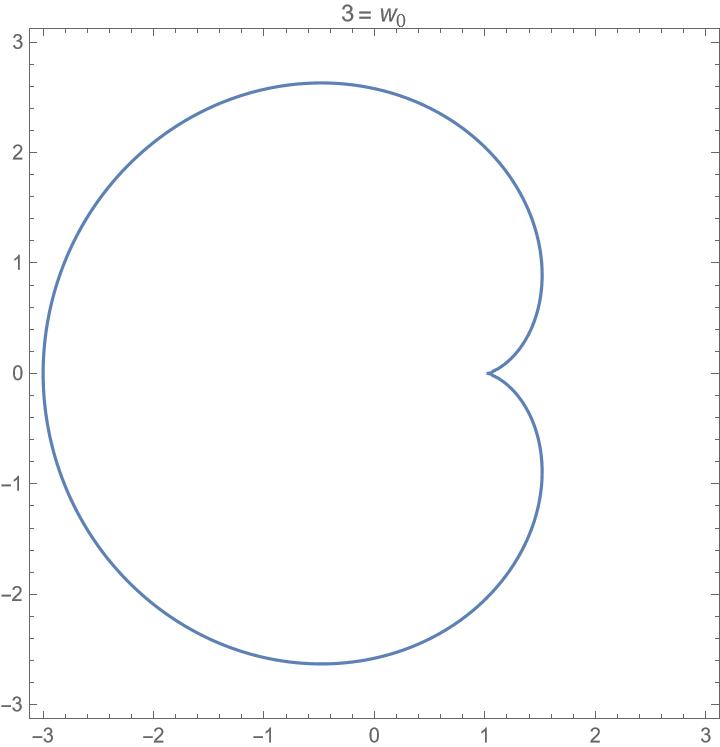
\includegraphics[width=.5\linewidth]{plots/1-1.jpg}
        \end{center}

        To find the direction of motion along the line, consider the point $U = -3$ and $V = 0$. Our system becomes
        \[ 
            \begin{cases}
                -16B_0^2 = V' < 0\\
                0 = U'
            \end{cases},
        \]
        and thus there is counterclockwise motion along the curve. Noting that there is a singularity $(1,0)$, we have that this is a one soliton case where the soliton for $U$ and $V$ look like

        \begin{center}
            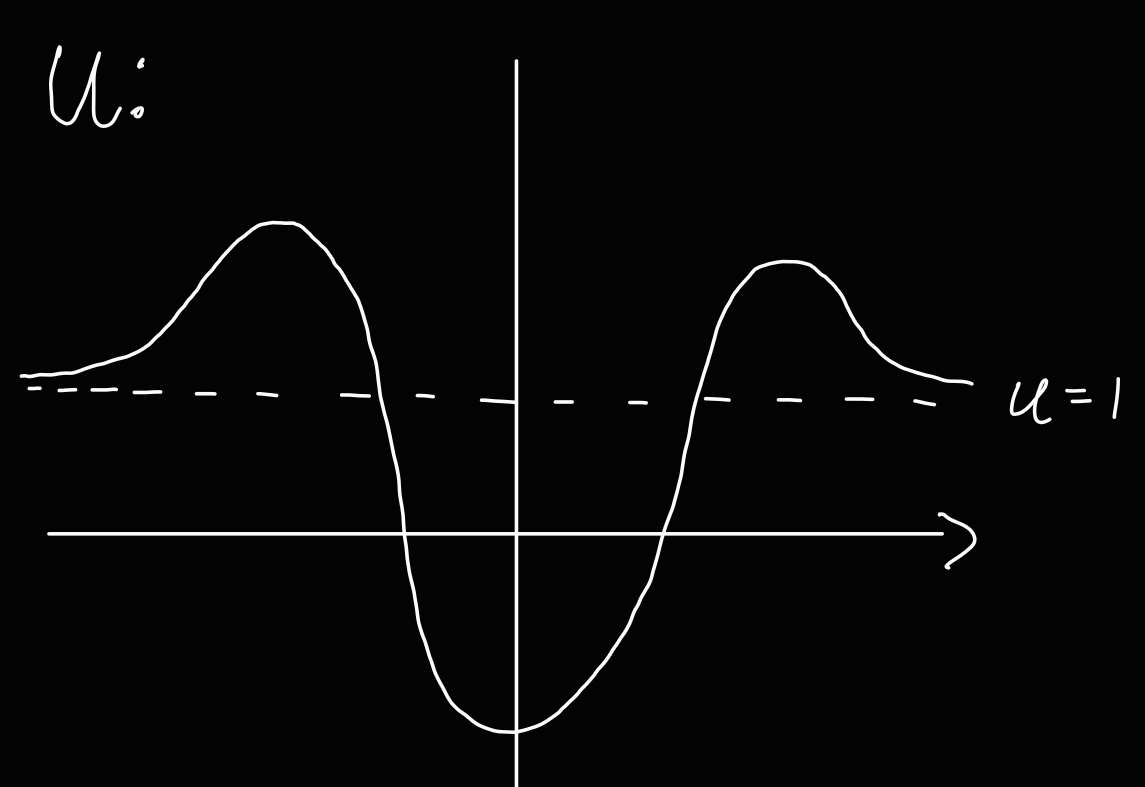
\includegraphics[width=.4\linewidth]{plots/fig1.jpg}
            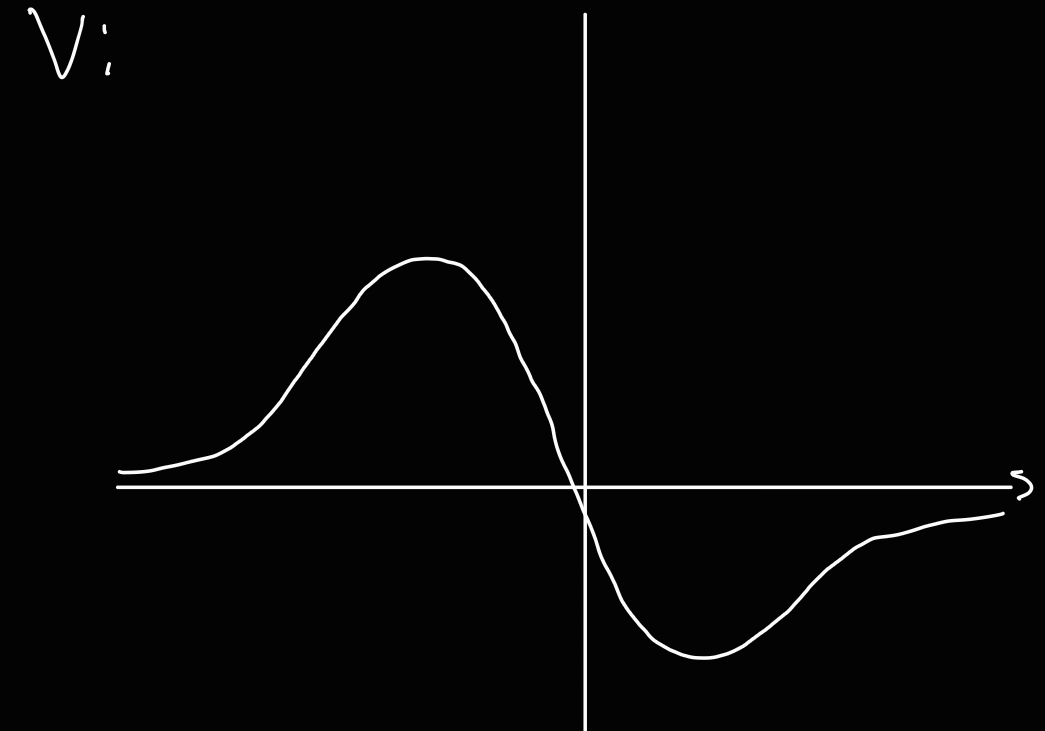
\includegraphics[width=.4\linewidth]{plots/fig2.jpg}
        \end{center}

        Note that it takes and infinite amount of time for $U$ to reach $U=1$ and $V$ and infinite amount of time to reach $V = 0$. 

        \noindent
        Now consider when $W_0 = 2$.
        \begin{center}
            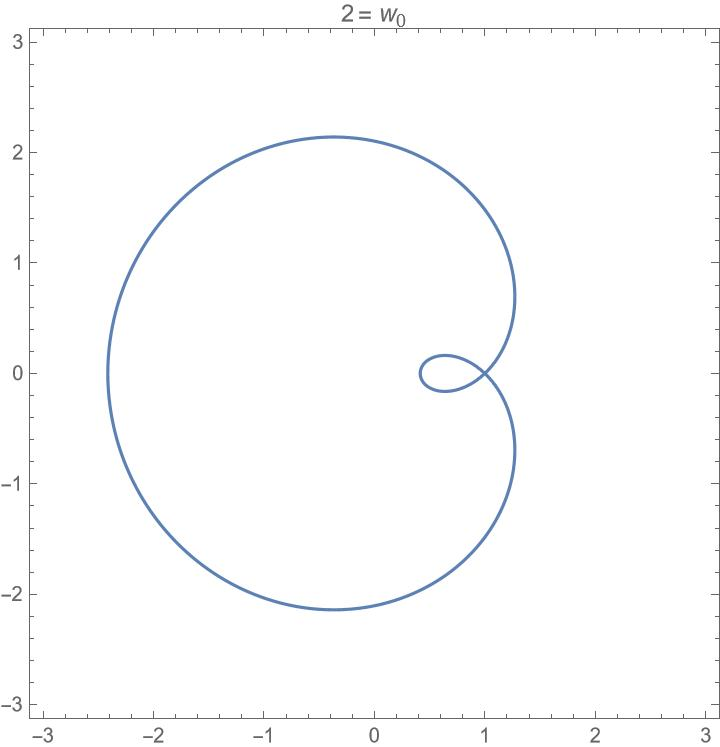
\includegraphics[width=.5\linewidth]{plots/1-2.jpg}
        \end{center}
        To find the direction of motion along the inner loop, consider the point $U=0$ and $V=0$. Our system becomes
        \[ 
            \begin{cases}
                B_0^2 = V' < 0\\
                0 = U'
            \end{cases},
        \]
        and thus the inner loop has clockwise motion. similarly we can verify that the outer loop has counterclockwise motion. In this case we have two solitons for $U$ and $V$. For the outer loop we have similar motion as in the previous case but with the maximums and minimum of $U$ and $V$ closer to the origin. The following plots show the soliton of $U$ and $V$ in the outer loop
        
        \begin{center}
            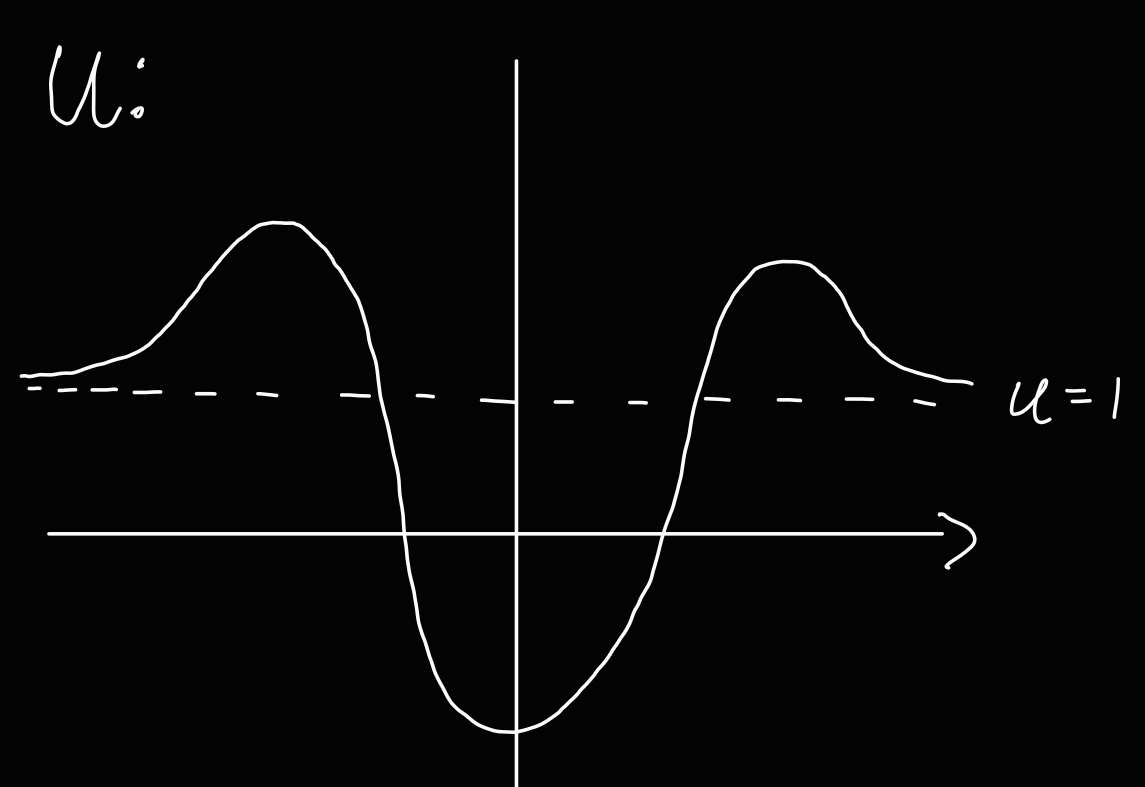
\includegraphics[width=.4\linewidth]{plots/fig1.jpg}
            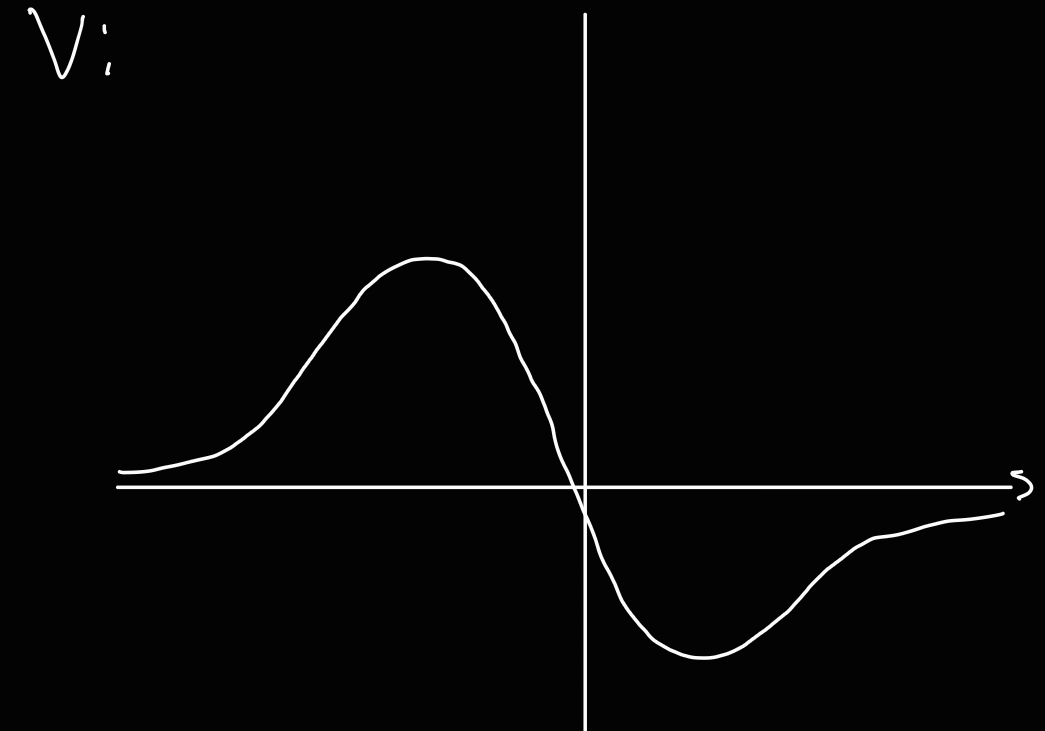
\includegraphics[width=.4\linewidth]{plots/fig2.jpg}
        \end{center}

        The following plots show the second soliton of $U$ and $V$ from the inner loop

        \begin{center}
            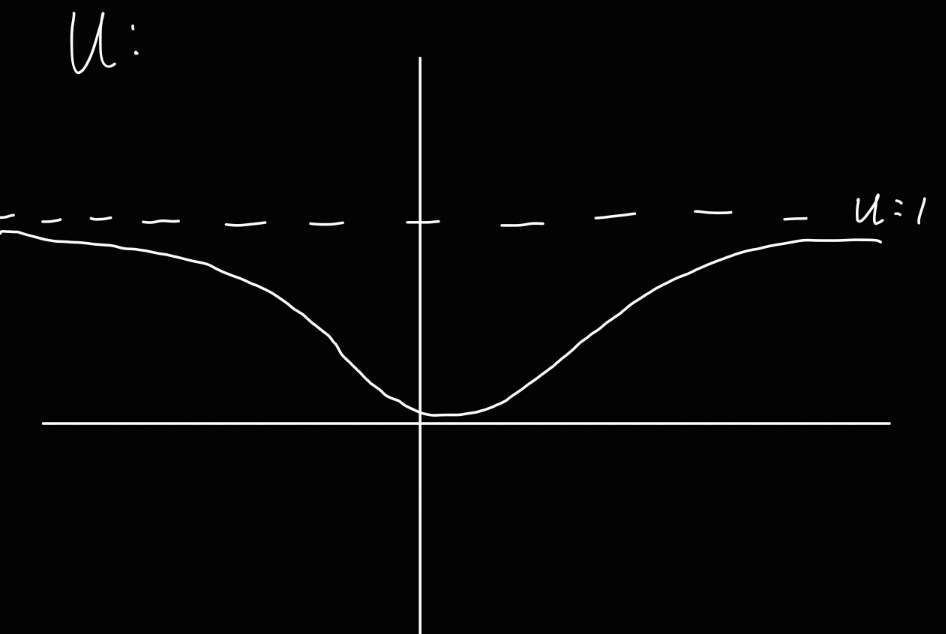
\includegraphics[width=.4\linewidth]{plots/fig3.jpg}
            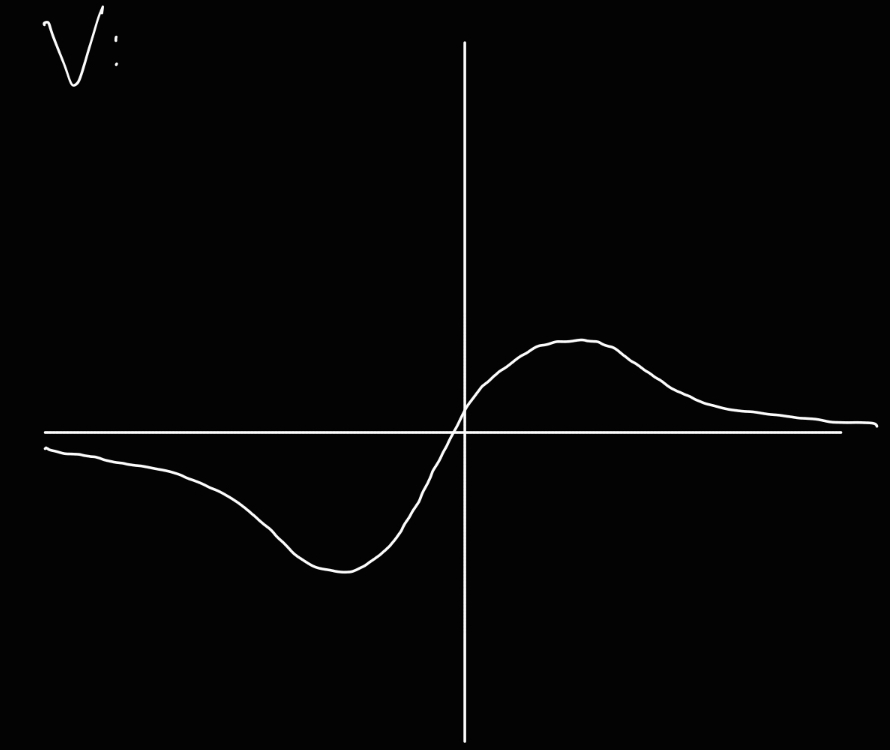
\includegraphics[width=.4\linewidth]{plots/fig4.jpg}
        \end{center}

        \noindent
        Now consider when $W_0 = 1.1$.
        \begin{center}
            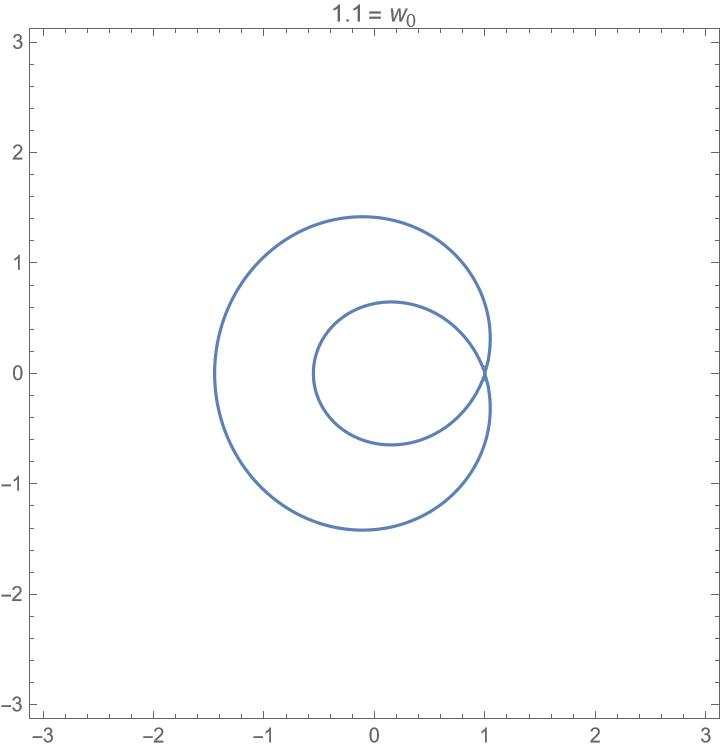
\includegraphics[width=.5\linewidth]{plots/1-3.jpg}
        \end{center}
        similarly to when $W_0 = 2$, we have the counterclockwise motion on the outer loop and clockwise motion in the inner. We have two solitons for $U$ and $V$ with similar behavior as before. Note that the max and min for the soliton of $U$ and $V$ corresponding to the outer loop is decreasing while the inner loop is increasing. The following figures show the soliton corresponding to the outer loop
        
        \begin{center}
            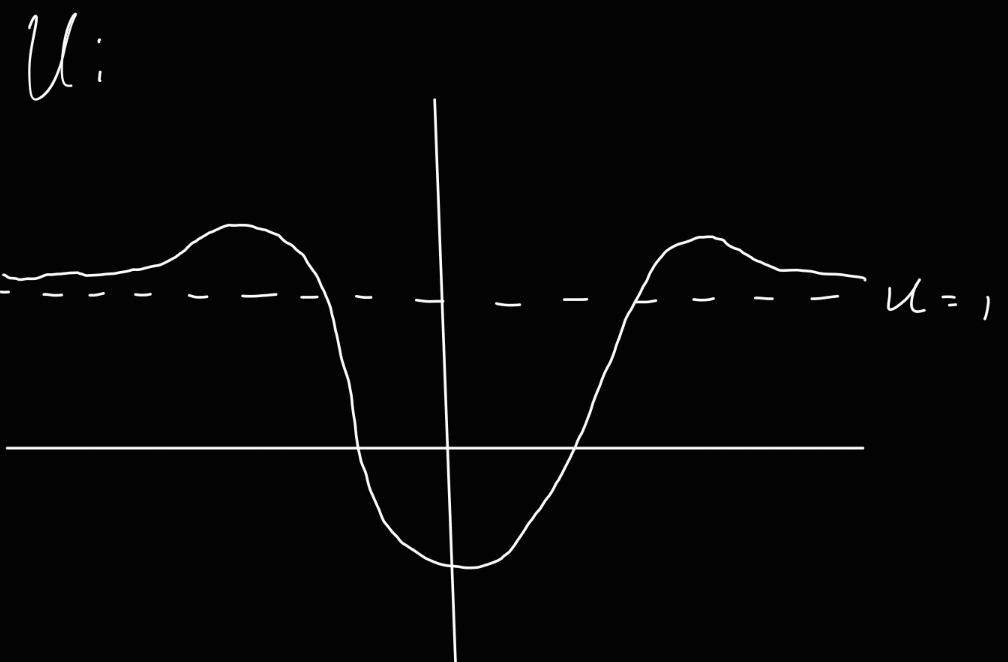
\includegraphics[width=.4\linewidth]{plots/fig5.jpg}
            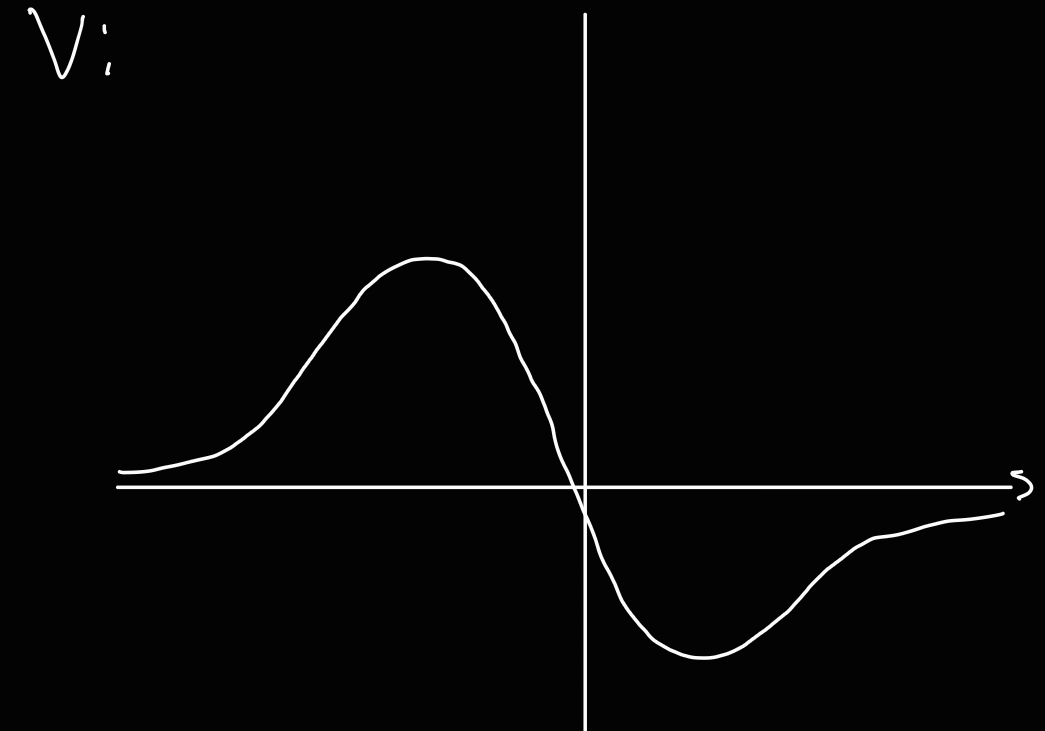
\includegraphics[width=.4\linewidth]{plots/fig2.jpg}
        \end{center}

        The following figures show the soliton corresponding to the inner loop
        \begin{center}
            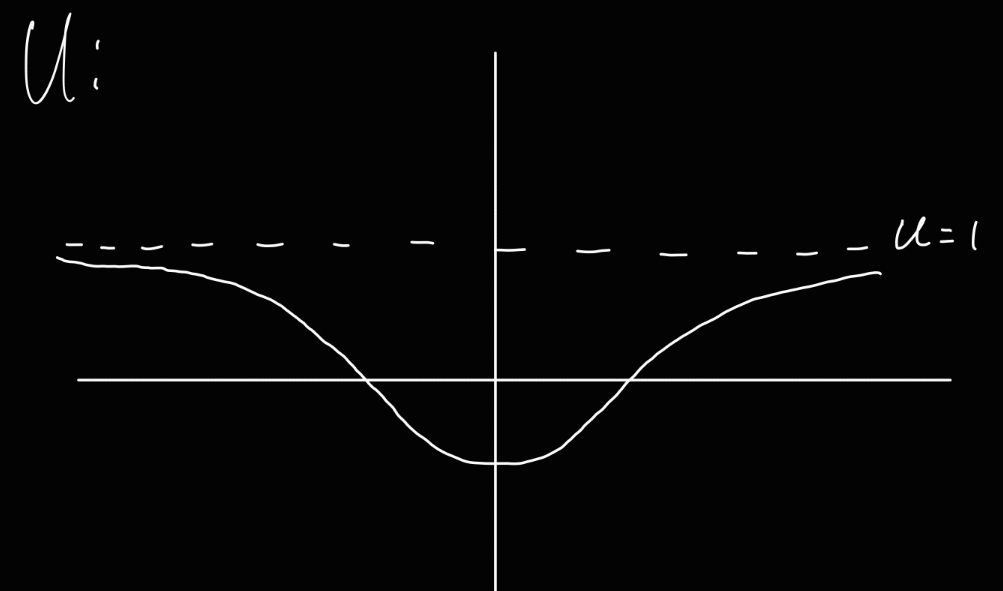
\includegraphics[width=.4\linewidth]{plots/fig6.jpg}
            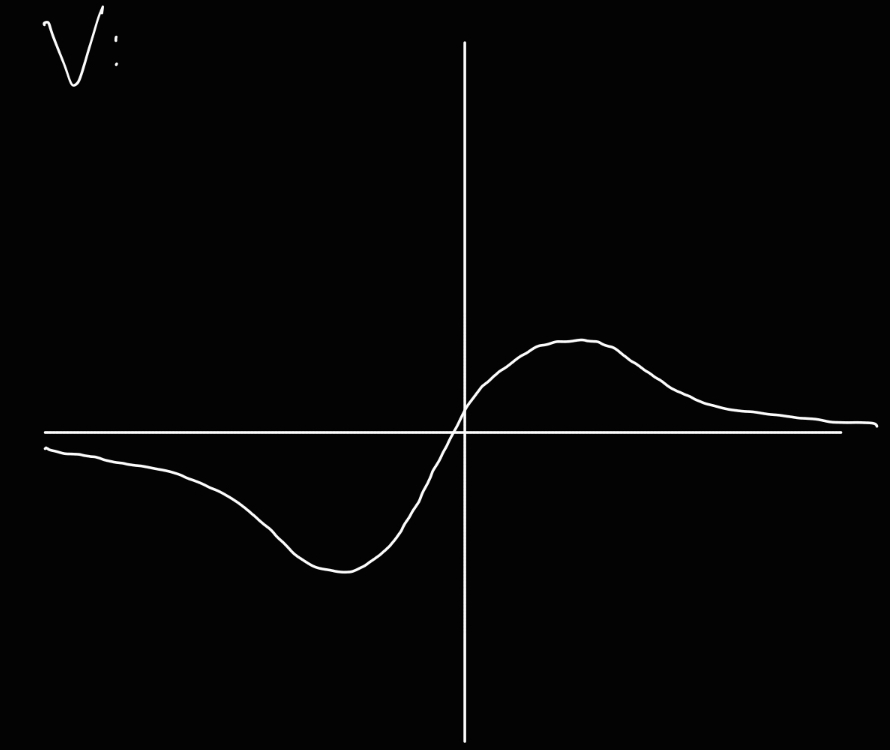
\includegraphics[width=.4\linewidth]{plots/fig4.jpg}
        \end{center}

        \noindent
        Now consider when $W_0 = 1$.
        \begin{center}
            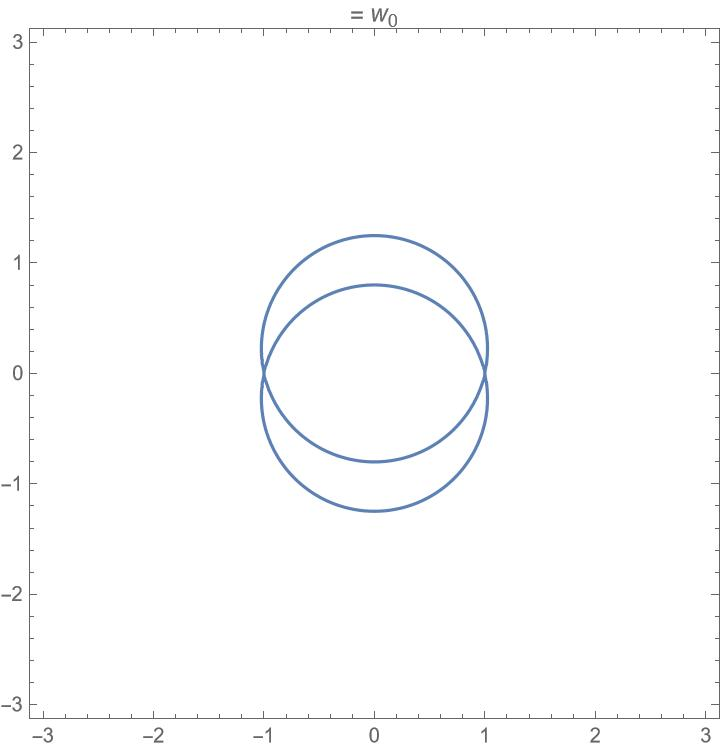
\includegraphics[width=.5\linewidth]{plots/1-4.jpg}
        \end{center}
        Notice that in this case we have two singularities at $\pm 1$. From the figure above, we see that $U$ has a heteroclinic orbit between $-1$ and $1$. But this means that the boundary condition that $U \to B_0$ as $|x| \to \infty$ is not met and thus this case does not satisfy the system's boundary condition. Therefore there are no solitons in this case for $U$ and $V$.  


        \noindent
        Now consider when $W_0 = 0.95$.
        \begin{center}
            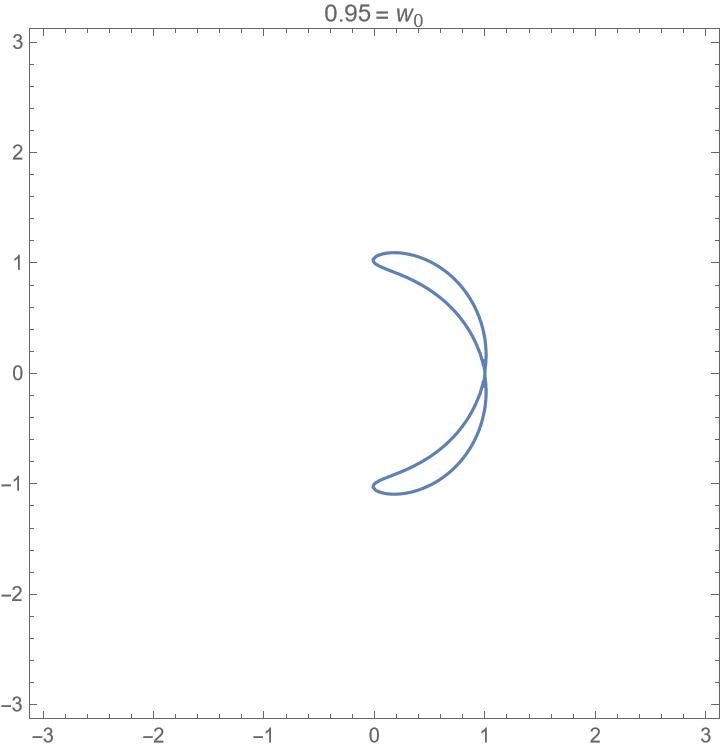
\includegraphics[width=.5\linewidth]{plots/1-5.jpg}
        \end{center}
        To find the direction of motion, consider the points $U = 0$ and $V=\pm 1$. From our system we get that $V' < 0$ and thus both the upper and lower loop have counterclockwise motion. This is a two soliton case and the following figures show the soliton of $U$ and $V$ for the upper loop

        \begin{center}
            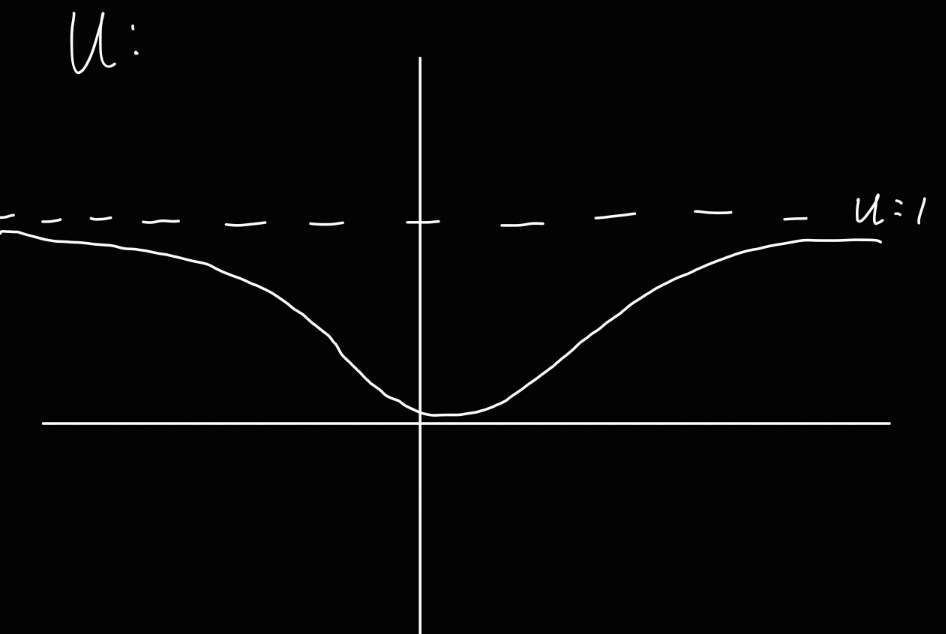
\includegraphics[width=.4\linewidth]{plots/fig3.jpg}
            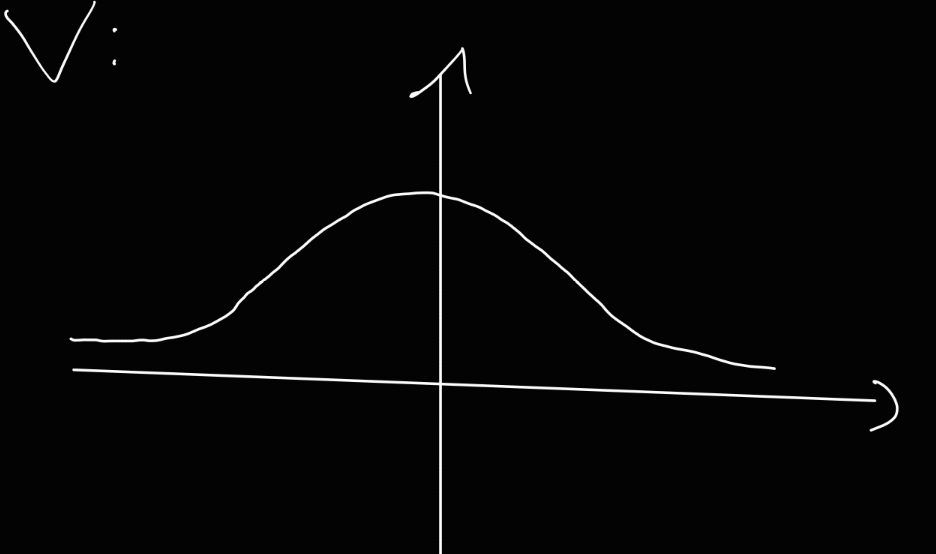
\includegraphics[width=.4\linewidth]{plots/fig7.jpg}
        \end{center}

        The following figures show the soliton of $U$ and $V$ for the lower loop

        \begin{center}
            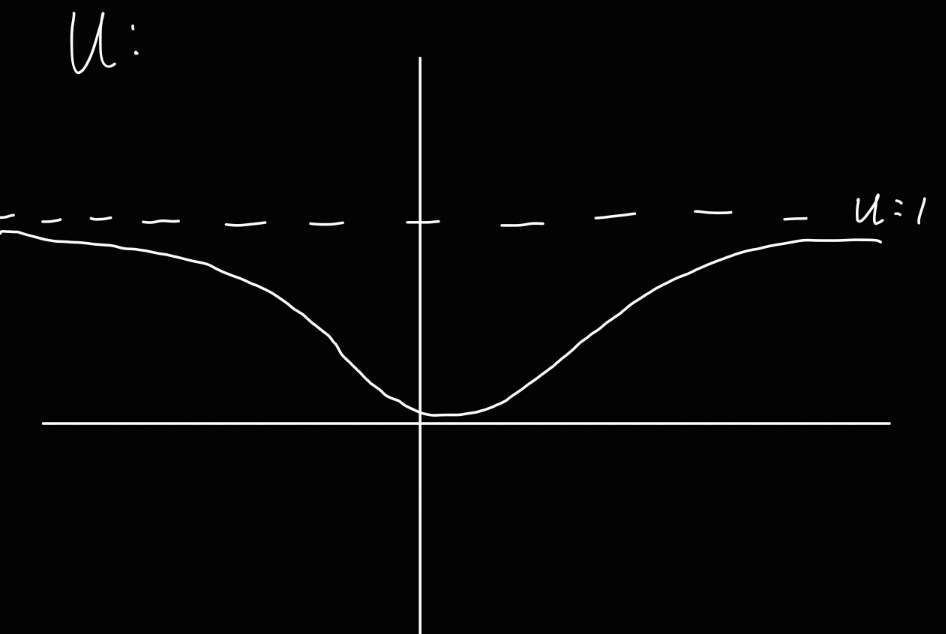
\includegraphics[width=.4\linewidth]{plots/fig3.jpg}
            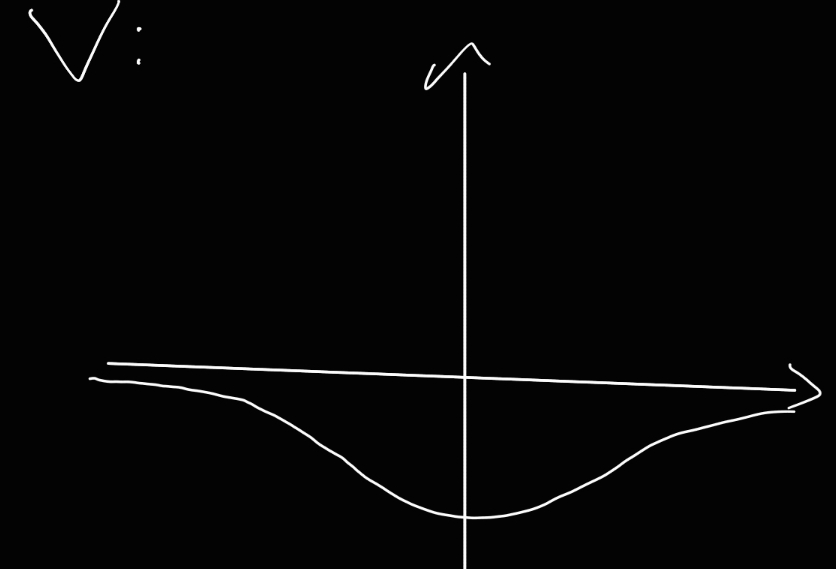
\includegraphics[width=.4\linewidth]{plots/fig8.jpg}
        \end{center}

        \noindent
        Now consider when $W_0 = 0.9$.
        \begin{center}
            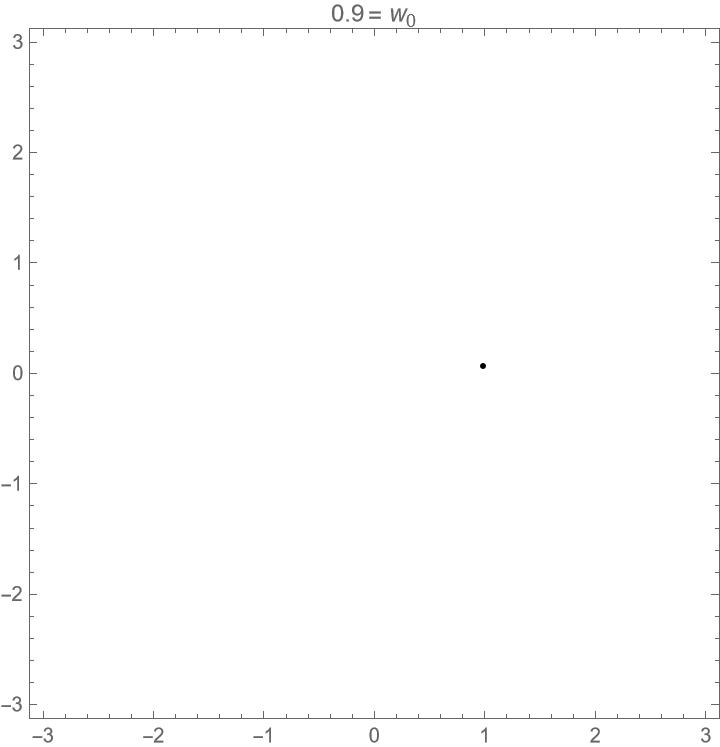
\includegraphics[width=.5\linewidth]{plots/1-6.jpg}
        \end{center}
        Since in this case we just have the singularity at $(0,1)$, we have no soliton solutions. 

    \end{enumerate}
    


\end{solution}

%----------------------------------------------------------------------------------------------------%
%\vskip 20pt
\newpage

%---------------%
%---Problem 2---%
%---------------%

%--Complete--$

\begin{problem}
    Show that the canonical Poisson bracket
$$\{f,g\}=\sum_{j=1}^N \left(\pp{f}{q_j}\pp{g}{p_j}-
\pp{f}{p_j}\pp{g}{q_j}\right)
$$
satisfies the Jacobi identity
$$
\{\{f,g\},h\}+\{\{g,h\},f\}+\{\{h,f\},g\}=0.
$$
\end{problem}

\begin{solution}

    \noindent
    Consider the canonical Poisson bracket
    \[
    \{f,g\}=\sum_{j=1}^N \left(\pp{f}{q_j}\pp{g}{p_j}-
    \pp{f}{p_j}\pp{g}{q_j}\right).
    \]
    We wish to show that
    \[
    \{\{f,g\},h\}+\{\{g,h\},f\}+\{\{h,f\},g\}=0.
    \]
    Observe that,
    \begin{align*}
        \{\{f,g\},h\} &=\sum_{i=1}^N\sum_{j=1}^N \pp{}{q_i}\paren{\pp{f}{q_j}\pp{g}{p_j} - \pp{f}{p_j}\pp{g}{q_j}}\pp{h}{p_i} - \pp{}{p_i}\paren{\pp{f}{q_j}\pp{g}{p_j} - \pp{f}{p_j}\pp{g}{q_j}}\pp{h}{q_i}\\
        &=\sum_{i=1}^N\sum_{j=1}^N \pp{f}{q_j}\pp{g}{q_i\partial p_j}\pp{h}{p_i} + \pp{g}{p_j}\pp{f}{q_i\partial q_j}\pp{h}{p_i} - \pp{f}{p_j}\pp{g}{q_i\partial q_j}\pp{h}{p_i}-\pp{g}{q_j}\pp{f}{q_i\partial p_j}\pp{h}{p_i}\\
        &-\pp{f}{q_j}\pp{g}{p_i\partial p_j}\pp{h}{q_i} - \pp{g}{p_j}\pp{f}{p_i \partial q_j}\pp{h}{g_i} + \pp{f}{p_j}\pp{g}{p_i\partial q_j}\pp{h}{q_i} + \pp{g}{q_j}\pp{f}{p_i \partial p_j}\pp{h}{q_i}\\
        \{\{g,h\},f\} &=\sum_{i=1}^N\sum_{j=1}^N \pp{}{q_i}\paren{\pp{g}{q_j}\pp{h}{p_j} - \pp{g}{p_j}\pp{h}{q_j}}\pp{f}{p_i} - \pp{}{p_i}\paren{\pp{g}{q_j}\pp{h}{p_j} - \pp{g}{p_j}\pp{h}{q_j}}\pp{f}{q_i}\\
        &=\sum_{i=1}^N\sum_{j=1}^N \pp{g}{q_j}\pp{h}{q_i\partial p_j}\pp{f}{p_i} + \pp{h}{p_j}\pp{g}{q_i\partial q_j}\pp{f}{p_i} - \pp{g}{p_j}\pp{h}{q_i\partial q_j}\pp{f}{p_i}-\pp{h}{q_j}\pp{g}{q_i\partial p_j}\pp{f}{p_i}\\
        &-\pp{g}{q_j}\pp{h}{p_i\partial p_j}\pp{f}{q_i} - \pp{h}{p_j}\pp{g}{p_i \partial q_j}\pp{f}{g_i} + \pp{g}{p_j}\pp{h}{p_i\partial q_j}\pp{f}{q_i} + \pp{h}{q_j}\pp{g}{p_i \partial p_j}\pp{f}{q_i}\\
        \{\{h,f\},g\} &=\sum_{i=1}^N\sum_{j=1}^N \pp{}{q_i}\paren{\pp{h}{q_j}\pp{f}{p_j} - \pp{h}{p_j}\pp{f}{q_j}}\pp{g}{p_i} - \pp{}{p_i}\paren{\pp{h}{q_j}\pp{f}{p_j} - \pp{h}{p_j}\pp{f}{q_j}}\pp{g}{q_i}\\
        &=\sum_{i=1}^N\sum_{j=1}^N \pp{h}{q_j}\pp{f}{q_i\partial p_j}\pp{g}{p_i} + \pp{f}{p_j}\pp{h}{q_i\partial q_j}\pp{g}{p_i} - \pp{h}{p_j}\pp{f}{q_i\partial q_j}\pp{g}{p_i}-\pp{f}{q_j}\pp{h}{q_i\partial p_j}\pp{g}{p_i}\\
        &-\pp{h}{q_j}\pp{f}{p_i\partial p_j}\pp{g}{q_i} - \pp{f}{p_j}\pp{h}{p_i \partial q_j}\pp{g}{g_i} + \pp{h}{p_j}\pp{f}{p_i\partial q_j}\pp{g}{q_i} + \pp{f}{q_j}\pp{h}{p_i \partial p_j}\pp{g}{q_i}.\\
    \end{align*}
    Thus we have that
    \begin{align*}
        &\{\{f,g\},h\} + \{\{g,h\},f\} + \{\{h,f\},g\}\\ 
        &=\sum_{i=1}^N\sum_{j=1}^N \left[ \pp{f}{q_j}\pp{g}{q_i\partial p_j}\pp{h}{p_i} + \pp{g}{p_j}\pp{f}{q_i\partial q_j}\pp{h}{p_i} - \pp{f}{p_j}\pp{g}{q_i\partial q_j}\pp{h}{p_i}-\pp{g}{q_j}\pp{f}{q_i\partial p_j}\pp{h}{p_i} \right.\\
        &-\pp{f}{q_j}\pp{g}{p_i\partial p_j}\pp{h}{q_i} - \pp{g}{p_j}\pp{f}{p_i \partial q_j}\pp{h}{g_i} + \pp{f}{p_j}\pp{g}{p_i\partial q_j}\pp{h}{q_i} + \pp{g}{q_j}\pp{f}{p_i \partial p_j}\pp{h}{q_i}\\
        &+\pp{g}{q_j}\pp{h}{q_i\partial p_j}\pp{f}{p_i} + \pp{h}{p_j}\pp{g}{q_i\partial q_j}\pp{f}{p_i} - \pp{g}{p_j}\pp{h}{q_i\partial q_j}\pp{f}{p_i}-\pp{h}{q_j}\pp{g}{q_i\partial p_j}\pp{f}{p_i}\\
        &-\pp{g}{q_j}\pp{h}{p_i\partial p_j}\pp{f}{q_i} - \pp{h}{p_j}\pp{g}{p_i \partial q_j}\pp{f}{g_i} + \pp{g}{p_j}\pp{h}{p_i\partial q_j}\pp{f}{q_i} + \pp{h}{q_j}\pp{g}{p_i \partial p_j}\pp{f}{q_i}\\
        &+\pp{h}{q_j}\pp{f}{q_i\partial p_j}\pp{g}{p_i} + \pp{f}{p_j}\pp{h}{q_i\partial q_j}\pp{g}{p_i} - \pp{h}{p_j}\pp{f}{q_i\partial q_j}\pp{g}{p_i}-\pp{f}{q_j}\pp{h}{q_i\partial p_j}\pp{g}{p_i}\\
        &\left. -\pp{h}{q_j}\pp{f}{p_i\partial p_j}\pp{g}{q_i} - \pp{f}{p_j}\pp{h}{p_i \partial q_j}\pp{g}{g_i} + \pp{h}{p_j}\pp{f}{p_i\partial q_j}\pp{g}{q_i} + \pp{f}{q_j}\pp{h}{p_i \partial p_j}\pp{g}{q_i} \right].\\
    \end{align*}
    Noticing that the bounds on both our summations are the same, we can cancel terms all of these terms to get zero. For example consider the first term 
    \[ \pp{f}{q_j}\pp{g}{q_i\partial p_j}\pp{h}{p_i}, \]
    which has a corresponding term
    \[ -\pp{h}{p_j}\pp{g}{p_i \partial q_j}\pp{f}{g_i}, \]
    and since the $1 \leq i \leq N$ and $1 \leq j \leq N$, these terms will completely cancel. This holds for the rest of the terms and thus we have that
    \[ \{\{f,g\},h\} + \{\{g,h\},f\} + \{\{h,f\},g\} = 0.\] 
\end{solution}

%----------------------------------------------------------------------------------------------------%
%\vskip 20pt
\newpage

%---------------%
%---Problem 3---%
%---------------%

%--complete--$

\begin{problem}
    Show that the Sine-Gordon equation
$$
u_{tt}-u_{xx}+\sin(u)=0
$$
is Hamiltonian with canonical Poisson structure and Hamiltonian
$$
H=\int \left(\frac{1}{2} p^2+\frac{1}{2}q_{x}^2+1-\cos(q)\right)dx,
$$
where $q=u$, and $p=u_t$.
\end{problem}

\begin{solution}

    \noindent
    Consider the Sine-Gordon equation
    \[ u_{tt} - u_{xx} + \sin(u) = 0.\]
    Let's assume that
    \[H = \frac{1}{2}p^2 + \frac{1}{2}q^2_x + 1 - \cos(q)dx,\]
    is a Hamiltonian of the Sine-Gordon equation where $q = u$ and $p = u_t$. We have that
    \[ \mathcal{H} = \int(\frac{1}{2}u_t^2 + \frac{1}{2}u^2_x + 1 - \cos(u)dx).\]
    Observe that
    \[ 
        \begin{pmatrix}
            q_t\\p_t
        \end{pmatrix} = \begin{pmatrix}
            0 & 1 \\ -1 & 0
        \end{pmatrix}\begin{pmatrix}
            \frac{\delta H}{\delta q}\\\frac{\delta H}{\delta p} 
        \end{pmatrix}\implies
        \begin{cases}
            q_t = \frac{\delta H}{\delta p}\\
            p_t = - \frac{\delta H}{\delta q}
        \end{cases}.
    \]
    Now we can directly compute $\frac{\delta H}{\delta p}$ and $\frac{\delta H}{\delta p}$ to be
    \[ 
        \frac{\delta H}{\delta p} = \pp{\mathcal{H}}{p} - \partial_x \pp{\mathcal{H}}{p_x} = p - \partial_x(0) = p = q_t = u_t,
    \]
    \[ 
        \frac{\delta H}{\delta q} = \sin(q) - \partial_x(q_x) = \sin(q) - q_{xx} = -p_t = -u_{tt}.
    \]
    And thus we have gotten the Sine-Gordon equation since 
    \[ 
       \sin(q) - q_{xx} = -u_{tt} \implies \sin(q) - u_{xx} = -u_{tt} \implies \sin(q) - u_{xx} + u_{tt} = 0.
    \]
    Therefore $H$ is indeed the Hamiltonian and the Sine-Gordon equation is Hamiltonian with canonical Poisson structure. 
\end{solution}

%----------------------------------------------------------------------------------------------------%
%\vskip 20pt
\newpage

%---------------%
%---Problem 4---%
%---------------%

%--Complete--$

\begin{problem}
    Check explicitly that the conserved quantities $F_{-1}=\int u dx$,
$F_0=\int \frac{1}{2} u^2 dx$,
$F_1=\int\left(\frac{1}{6}u^3-\frac{1}{2}u_x^2\right) dx$, $F_2=\int
\left(\frac{1}{24}u^4-\frac{1}{2}uu_x^2+\frac{3}{10}u_{xx}^2\right)dx$ are
mutually in involution with respect to the Poisson bracket defined by the
Poisson structure given by $\partial_x$.
\end{problem}

\begin{solution}

    \noindent
    We wish to show that $F_{-1}=\int u dx$,
    $F_0=\int \frac{1}{2} u^2 dx$,
    $F_1=\int\left(\frac{1}{6}u^3-\frac{1}{2}u_x^2\right) dx$, 
    
    \noindent
    $F_2=\int \left(\frac{1}{24}u^4-\frac{1}{2}uu_x^2+\frac{3}{10}u_{xx}^2\right)dx$ are mutually in involution with respect to the Poisson bracket defined by the Poisson structure given by $\partial_x$. Note that
    \[ \{F_i,F_j\} = 0 \implies \{F_j,F_i\} = 0 ~\text{as}~\{F_i,F_j\} = - \{F_j,F_i\},\]
    since the Poisson bracket is antisymmetric.
    Next observe that $\{F_i,F_{-1}\} = 0$ for all $i$ since 
    \[ \partial_x(\frac{\delta}{\delta u}u) = \partial_x 1 = 0.\]
    Thus $F_{-1}$ is mutually an involution with $F_0,F_1,$ and $F_2$.
    Next note that 
    \[\{F_i,F_j\} =0 \iff \frac{\delta}{\delta u}\paren{\frac{\delta F_i}{\delta u} \partial_x \frac{\delta F_j}{\delta u}} = 0.\]
    Thus we can check that the rest are involutions by computing $\frac{\delta}{\delta u}\paren{\frac{\delta F_i}{\delta u} \partial_x \frac{\delta F_j}{\delta u}}$ and verifying it to equal zero. We used Mathematica and the package \verb+VariationalMethods+ to compute the variationally derivatives. We found that $\frac{\delta}{\delta u}\paren{\frac{\delta F_0}{\delta u} \partial_x \frac{\delta F_1}{\delta u}} = 0$ which implies that $\{F_0,F_1\} = 0$, and similarly we verified that $\{F_0,F_2\} = 0,$ and $\{F_1,F_2\} = 0.$ Thus we have that $F_{-1},F_0,F_1,$ and $F_2$ are mutually involutions with respect to the Poisson bracket.

\end{solution}

%----------------------------------------------------------------------------------------------------%
%\vskip 20pt
\newpage

%---------------%
%---Problem 5---%
%---------------%

%--Complete--$

\begin{problem}
    Find the fourth conserved quantity for the KdV equation $u_t=u u_x+u_{xxx}$, $i.e.$, the conserved quantity which contains $\frac{1}{24} \int u^4 dx$.
\end{problem}

\begin{solution}

    \noindent
    We wish to find the fourth conserved quantity for the KdV equation
    \[ 
        u_t = uu_x + u_{xxx}.
    \] 
    Recall that we computed up to $[f]=6$ to find the third conserved quantity. We also know that there are only conserved quantities for even weights, so let's begin examining $[f]=8$. When $[f] = 8$, then the possible terms are $u^4,u^2u_{xx},uu_x^2,u_{xx}^2,u_xu_{xxx},uu_{4x},$ and $u_{6x}.$ We note that $u^2u_{xx}$ and $uu_{x}^2$ are equivalent and same with $u_xu_{xxx},uu_{4x},$ and $u_{8x}$. Thus let's consider
    \[
        f = a_1u^4 + a_2uu_x^2 + a_3u^2_{xx}.
    \] 
    We also need for $[g]=10$. The possible terms for this are $u^5,u^3u_{xx},u^2u_x^2,u^2u_{4x},uu_xu_{xxx},uu_{xx}^2,$ $u^2_xu_{xx}, uu_{6x},u_xu_{5x},u_{xx}u_{4x},u^2_{xxx},$ and $u_{5x}.$ This gives that
    \begin{align*}
        g&=c_1u^5 + c_2u^3u_{xx} + c_3u^2u_x^2 + c_4u^2u_{4x} + c_5uu_xu_{xxx} + c_6uu_{xx}^2 + c_7u_x^2u_{xx}\\ 
        &+ c_8uu_{6x} + c_9u_xu_{5x} + c_{10}u_{xx}u_{4x} + c_{11}u_{xxx}^2 + c_{12}u_{8x}.
    \end{align*} 
    Now we wish to compute $f_t + g_x$ so lets compute
    \[ 
        f_t = \frac{1}{6}u^3u_t + 2a_1uu_xu_{xt} + a_1u_tu_x^2 + 2a_2u_{xx}u_{xxt},
    \]
    and note that we can eliminate the time derivatives in $f_t$ using
    \begin{align*}
        u_t &= uu_x + u_{xxx}\\
        \implies u_{xt} &= \partial_x(uu_x + u_{xxx})\\
        \implies u_{xxt} &= \partial_{xx}(uu_x + u_{xxx}).
    \end{align*}
    Plugging these into Mathematica and computing $f_t + g_t$, we can find the following system of equations by looking at the coefficients 
    \begin{align*}
        u^4u_x&: ~~ -\frac{1}{6} + \frac{30}{6}c_1 = 0\\
        u^3u_{3x}&: ~~ -\frac{1}{6} + c_2 = 0\\
        u_x^2u_{5x}&: ~~-a_1 + c_5 + c_7 = 0\\
        u_{3x}u_{4x}&: ~~c_{10}+2c_{11}\\
        u_{2x}u_{5x}&: ~~ -2a_2 + c_10 + c_9\\
        u^2u_xu_{xx}&: ~~ -2a_1 + 3c_2 + 2c_3\\
        u^2u_{5x}&: ~~ c_4 = 0\\
        u_xu_{xx}^2&: ~~ -6a_2 + c_6 + 2c_7\\
        u_xu_{6x}&: ~~ c_8 + c_9 = 0\\
        uu_x^3&: ~~ -3a_1 + 2c_3 = 0\\
        uu_{xx}u_{xxx}&: ~~ -2a_2 + c_5 + 2c_6 = 0\\
        uu_xu_{4x}&: ~~ -2a_1 + 2c_4 + c_5 = 0\\
        u_{7x}&: ~~ c_8 = 0\\
        u_{9x}&: ~~ c_{12} = 0. 
    \end{align*}
    Simplifying this system gives
    \begin{align*}
        a_1 &= c_5 + c_7\\
        a_1 &= \frac{1}{4} + c_3\\
        a_1 &= \frac{2}{3}c_3\\
        a_1 &= \frac{1}{2}c_5\\
        a_2 &= \frac{1}{2}c_{10}\\
        a_2 &= \frac{1}{6}c_6 + \frac{1}{3}c_7\\
        a_2 &= \frac{1}{2}c_5 + c_6
    \end{align*}
    Solving this system gives
    \[ 
        a_1 = -\frac{1}{2}, ~~\text{and}~~ a_2 = \frac{3}{10}.
    \]
    Thus we have found the fourth conserved quantity of the KdV equation to be
    \[ 
        \int \paren{\frac{1}{24}u^4 - \frac{1}{2}uu_x^2 + \frac{3}{10}u_{xx}^2}dx.
    \]

\end{solution}

%----------------------------------------------------------------------------------------------------%
%\vskip 20pt
\newpage

%---------------%
%---Problem 6---%
%---------------%

%--Complete--$

\begin{problem}
    {\bf Recursion operator} For a Bi-Hamiltonian system with two Poisson
structures given by $B_0$, $B_1$, one defines a recursion operator $R=B_1
B_0^{-1}$, which takes one element of the hierarchy of equations to the next
element. For the KdV equation with $B_0=\partial_x$ and $B_1=
\partial_{xxx}+\frac{1}{3}(u\partial_x+\partial_x u)$, we get $B_0^{-1}=\partial_x^{-1}$, integration with
respect to x. Write down the recursion operator. Apply it to $u_x$ (the zero-th
KdV flow)  to obtain the first KdV flow. Now apply it to $uu_x+u_{xxx}$ to get
(up to rescaling of $t_2$) the second KdV equation. What is the third KdV
equation?
\end{problem}

\begin{solution}

    \noindent
    Consider a Bi-Hamiltonian system for the KdV equation with two Poisson structures given by $B_0 = \partial_x$ and $B_1=\partial_{xxx}+\frac{1}{3}(u\partial_x+\partial_x u)$ where $R = B_1B_0^{-1}$ defines the recursion operator. First let's explicitly compute the recursion operator
    \begin{align*}
        R = B_1B_0^{-1} &= (\partial_{xxx}+\frac{1}{3}u\partial_x+ \frac{1}{3}\partial_x u)(\partial_x^{-1})\\
        &= \partial_{xxx}\partial_x^{-1}+\frac{1}{3}u\partial_x\partial_x^{-1}+ \frac{1}{3}\partial_x u\partial_x^{-1}\\
        &= \partial_{xx}+\frac{1}{3}u+ \frac{1}{3}\partial_x u\partial_x^{-1},\\
    \end{align*} 
    where $B_0^{-1} = \partial_x^{-1} = \int dx.$ Now we wish to apply $R$ to $u_x$ to obtain the first KdV flow
    \begin{align*}
        Ru_x &= (\partial_{xx}+\frac{1}{3}u+ \frac{1}{3}\partial_x u\partial_x^{-1})u_x\\
        &=u_{xxx} + \frac{1}{3}uu_x + \frac{1}{3}\partial_x u \partial_x^{-1}u_x\\
        &=u_{xxx} + \frac{1}{3}uu_x + \frac{1}{3}\partial_x u^2\\
        &=u_{xxx} + \frac{1}{3}uu_x + \frac{2}{3}uu_x\\
        &=u_{xxx} + uu_x.
    \end{align*}
    Thus $u_{xxx} + uu_x$ is the first KdV flow. Now we wish to apply $R$ to the first KdV flow to find the second KdV equation
    \begin{align*}
        R(u_{xxx} + uu_x) &= (\partial_{xx}+\frac{1}{3}u+ \frac{1}{3}\partial_x u\partial_x^{-1})(u_{xxx} + uu_x)\\
        &= \partial_x(uu_{xx} + u_xu_x) + \frac{1}{3}u^2u_x + \frac{1}{3}\partial_x u \partial_x^{-1}\paren{\frac{1}{2}u^2}_x + u_{5x} + \frac{1}{3}uu_{xxx}+ \frac{1}{3}\partial_x(uu_{xx})\\
        &= uu_{xxx} + u_xu_{xx} + 2u_xu_{xx} + \frac{1}{3}u^2u_x + \frac{1}{2}u^2u_x + u_{5x} + \frac{1}{3}uu_{xxx} + \frac{1}{3}uu_{xxx} + \frac{1}{3}u_xu_{xx}\\
        &=\frac{5}{3}uu_{xxx} + \frac{10}{3}u_xu_{xx} + \frac{5}{6}u^2u_x + u_{5x}.
    \end{align*}
    Thus we have found the second KdV equation. Now we wish to compute the third KdV equation by applying $R$ to the second KdV equation
    \begin{align*}
        &R\paren{\frac{5}{3}uu_{xxx} + \frac{10}{3}u_xu_{xx} + \frac{5}{6}u^2u_x + u_{5x}} = \paren{\partial_{xx}+\frac{1}{3}u+ \frac{1}{3}\partial_x u\partial_x^{-1}}\paren{\frac{5}{3}uu_{xxx} + \frac{10}{3}u_xu_{xx} + \frac{5}{6}u^2u_x + u_{5x}}\\
        &= \frac{5}{3}\partial_x (uu_{4x} + u_{xxx}u_x) + \frac{5}{9}u^2u_{xxx} + \frac{5}{9}\partial_x u \partial_x^{-1}(uu_{xx} - \frac{1}{2}u_x^2)_x + \frac{10}{3}\partial_x(u_xu_{xxx} + u_{xx}^2) + \frac{10}{9}uu_xu_{xx}\\ 
        &+ \frac{10}{9}\partial_x u \partial_x^{-1}\paren{\frac{1}{2}u_x^2}_x + \frac{5}{6}\partial_x(u^2u_{xx} + 2uu_x^2) + \frac{5}{18}u^3u_x + \frac{5}{18}\partial_x u \partial_x^{-1}\paren{\frac{1}{3}u^3}_x + u_{7x} + \frac{1}{3}uu_{5x} + \frac{1}{3}\partial_x(uu_{4x})\\
        &= \frac{5}{3}uu_{5x} + \frac{5}{3}u_xu_{4x} + \frac{5}{3}u_{xx}u_{xxx} + \frac{5}{3}u_xu_{4x} + \frac{5}{9}u^2u_{xxx} + \frac{5}{9}u^2u_{xxx} + \frac{10}{9}uu_xu_{xx} - \frac{10}{18}uu_xu_{xx} - \frac{5}{18}u_x^3 \\
        &+ \frac{10}{3}u_xu_{4x} + \frac{10}{3}u_{xx}u_{xxx} + \frac{20}{3}u_{xx}u_{xxx} + \frac{10}{9}uu_xu_{xx} + \frac{20}{18}uu_xu_{xx} + \frac{10}{18}u_x^3 + \frac{5}{6}u^2u_{xxx} + \frac{10}{6}uu_xu_{xx}\\ 
        &+ \frac{10}{3}uu_xu_{xx} + \frac{5}{3}u^3_x + \frac{5}{18}u^3u_x + \frac{20}{54}u^3u_x + u_{7x} + \frac{1}{3}uu_{5x} + \frac{1}{3}uu_{5x} + \frac{1}{3}u_xu_{4x}\\
        &=u_{7x} + \paren{\frac{5}{3} + \frac{1}{3} + \frac{1}{3}}uu_{5x} + \paren{\frac{5}{3} + \frac{5}{3} + \frac{10}{3} + \frac{1}{3}}u_xu_{4x} + \paren{\frac{5}{3} + \frac{10}{3} + \frac{20}{3}}u_{xx}u_{xxx} + \paren{\frac{5}{18} + \frac{20}{54}}u^3u_x\\ 
        &+ \paren{\frac{5}{9} + \frac{5}{9} + \frac{5}{6}}u^2u_{xxx} +\paren{\frac{10}{9} - \frac{10}{18} + \frac{18}{9} + \frac{20}{18} + \frac{10}{6} + \frac{10}{3}}uu_xu_{xx} + \paren{\frac{10}{18} + \frac{5}{3}-\frac{5}{18}}u_x^3\\
        &=u_{7x} + \frac{7}{3}uu_{5x} + 7u_xu_{4x} + \frac{35}{3}u_{xx}u_{xxx} + \frac{35}{18}u^2u_{xxx} + \frac{70}{9}uu_xu_{xx} + \frac{35}{18}u_x^3 + \frac{35}{54}u^3u_x.
    \end{align*}
    Thus we have found the third KdV equation.
\end{solution}

%----------------------------------------------------------------------------------------------------%
%\vskip 20pt
\newpage

%---------------%
%---Problem 7---%
%---------------%

%--Complete--$

\begin{problem}
    Consider the function $U(x)=2\partial_x^2\ln\left(1+e^{kx+\alpha}\right)$.
Show that for a suitable $k$, $U(x)$ is a solution of the first member of the
stationary KdV hierarchy (as you've already seen, it is the one-soliton
solution):

$$
6uu_x+u_{xxx}+c_0 u_x=0.
$$

\noindent (Note: it may be easier to define $c_0$ in terms of $k$, instead of
the other way around)

\noindent Having accomplished this, let
$u(x,t_1,t_2,t_3,\ldots)=U(x)|_{\alpha=\alpha(t_1,t_2,t_3,\ldots)}$. Determine
the dependence of $\alpha$ on $t_1$, $t_2$ and $t_3$ such that
$u(x,t_1,t_2,t_3,\ldots)$ is simultaneously a solution of the first, second and
third KdV equations:
\begin{align*}
    u_{t_1}&=6 u u_x+u_{xxx},\\
    u_{t_2}&=30u^2u_x+20u_x u_{xx}+10u u_{xxx}+u_{5x},\\
    u_{t_3}&=140 u^3 u_x+70 u_x^3+280 u u_x u_{xx}+70 u_{xx}u_{xxx}+70
    u^2 u_{xxx}+42u_x u_{xxxx}+14 u u_{5x}+u_{7x}.
\end{align*}

\noindent Based on this, write down a guess for the one-soliton solution that solves the entire KdV hierarchy.
\end{problem}

\begin{solution}

    \noindent
    Consider the function $U(x) = 2\partial_x^2\ln\left(1+e^{kx+\alpha}\right)$. We wish to show that for a suitable $k$, $U(x)$ is a solution to the first member of the stationary KdV hierarchy
    \[ 6uu_x + u_{xxx} + c_0u_x = 0.\]
    Using Mathematica, we plugged $U(x)$ into the first KdV equation to get
    \[ 0 = - \frac{2 e^{k x + \alpha} \paren{-1 + e^{k x + \alpha}}k^3(k^2+c_0)}{(1 + e^{k x + \alpha})^3},\]
    which holds when $k^2 = -c_0$. 
    
    \noindent
    Next let $u(x,t1,t2,t3,\ldots) = \left. U(x) \right|_{\alpha = \alpha(t_1,t_2,t_3,\ldots)}$. We wish to determine the dependence of $\alpha$ on $t_1, t_2,$ and $t_3$ such that $u(x,t_1,t_2,t_3,\ldots)$ is simultaneously a solution to the first, second, and third KdV equations. Using Mathematica, we plugged
    \begin{align}
        u(x,t1,t2,t3) = 2\partial_x^2\ln\left(1+e^{kx+\alpha(t_1,t_2,t_3)}\right),
    \end{align} 
    into the first KdV equation
    \[ 
        0 = - u_{t_1} + 6 u u_x+u_{xxx},
    \]
    which gives
    \[ 
        0 = 4k^2\text{csch}(kx + \alpha)^3\sinh\paren{\frac{1}{2}(kx + \alpha)}^4 (-k^3 + \alpha_{t_1}).
    \]
    To satisfy this equality, we require $\alpha_{t_1} = k^3$.

    \noindent
    Next we plugged (1) into the second KdV equation
    \[ 
        0=- u_{t_2} + 30u^2u_x+20u_x u_{xx}+10u u_{xxx}+u_{5x}
    \]
    which gives
    \[ 
        0 = 4k^2\text{csch}(kx + \alpha)^3\sinh\paren{\frac{1}{2}(kx + \alpha)}^4 (-k^5 + \alpha_{t_2}).
    \]
    To satisfy this equality, we require $\alpha_{t_2} = k^5$.

    \noindent
    Finally we plugged (1) into the third KdV equation
    \[ 
        0= - u_{t_3} + 140 u^3 u_x+70 u_x^3+280 u u_x u_{xx}+70 u_{xx}u_{xxx}+70 u^2 u_{xxx}+42u_x u_{xxxx}+14 u u_{5x}+u_{7x},
    \]
    which gives
    \[ 
        0 = 4k^2\text{csch}(kx + \alpha)^3\sinh\paren{\frac{1}{2}(kx + \alpha)}^4 (-k^5 + \alpha_{t_3}).
    \]
    To satisfy this equality, we require $\alpha_{t_3} = k^7$. Thus we see a pattern in the $\alpha$ dependence on $t_1,t_2,\ldots$ to be
    \[ \alpha_{t_n} =k^{1 + 2n}.\]
    Therefore, I'd guess that a one-soliton solution that solves the entire KdV hierarchy is given by
    \[ 
        u(x,t_1,t_2,t_3,\ldots) = 2\partial_x^2\ln\left(1+e^{kx+\alpha}\right),
    \]
    where
    \[ 
        \alpha = k^3t_1 + k^5t_2 + \cdots + k^{1+2n}t_n + \cdots.
    \]


\end{solution}

%----------------------------------------------------------------------------------------------------%
%\vskip 20pt
\newpage

%---------------%
%---Problem 8---%
%---------------%

%--Complete--$

\begin{problem}
    {\bf Warning: maple/mathematica-intensive.} Consider the function
$$
U(x)=2\partial_x^2\ln\left(1+e^{k_1
x+\alpha}+e^{k2_x+\beta}+\left(\frac{k_1-k_2}{k_1+k_2}\right)^2
e^{k_1x+k_2 x+\alpha+\beta}\right).
$$
Show that for a suitable $k_1$, $k_2$,
$U(x)$ is a solution of the second member of the stationary KdV hierarchy:

$$
30u^2u_x+20u_x u_{xx}+10u u_{xxx}+u_{5x}+c_1(6uu_x+u_{xxx})+c_0 u_x=0.
$$

\noindent (Note: it may be easier to define $c_1$, $c_0$ in terms of $k_1$ and
$k_2$ instead of the other way around)

\noindent Having accomplished this, let
$u(x,t_1,t_2,t_3,\ldots)=U(x)|_{\alpha=\alpha(t_1,t_2,t_3,\ldots),
\beta=\beta(t_1,t_2,t_3,\ldots)}$. Determine
the dependence of $\alpha$ and $\beta$ on $t_1$, $t_2$ and $t_3$ such that
$u(x,t_1,t_2,t_3,\ldots)$ is simultaneously a solution of the first, second and
third KdV equations, given above.

Based on this, write down a guess for the two-soliton solution of
the entire KdV hierarchy. 
\end{problem}

\begin{solution}
    
    \noindent
    Consider the function
    \[ 
        U(x)=2\partial_x^2\ln\left(1+e^{k_1
x+\alpha}+e^{k2_x+\beta}+\left(\frac{k_1-k_2}{k_1+k_2}\right)^2
e^{k_1x+k_2 x+\alpha+\beta}\right).
    \]
    We first wish to show that for a suitable $k_1$ and $k_2$, $U(x)$ is a solution of the second member of the stationary KdV hierarchy
    \[ 
        30u^2u_x+20u_x u_{xx}+10u u_{xxx}+u_{5x}+c_1(6uu_x+u_{xxx})+c_0 u_x=0.
    \]
    Using Mathematica, we plugged $U(x)$ into the second KdV equation resulting in am extremely long expression involving many fractions. To simplify the problem, I used Mathematica's \verb+Together+ function to get a common denominator. Since we are looking for when this fraction will be zero, I used Mathematica's \verb+Numerator+ to get the numerator of the fraction. Finally I arbitrarily picked two terms from the numerator and used Mathematica's \verb+Solve+ to solve the two by two system created by the coefficients of the two terms for $c_0$ and $c_1$. If the solve function was unable to find a solution, I picked two other terms. Once I got a solutions, I plugged them back into the original equation to verify that $U(x)$ with the new values. If the new values didn't zero $U(x)$, I picked two new terms and repeated the process. Using this method I found that $U(x)$ satisfies the second KdV equation when $c_0 = k_1^2k_2^2$ and $c_1 = -k_1^2-k_2^2.$ 
    
    \noindent 
    Next let $u(x,t_1,t_2,t_3,\ldots)=U(x)|_{\alpha=\alpha(t_1,t_2,t_3,\ldots),
    \beta=\beta(t_1,t_2,t_3,\ldots)}$. We wish to determine
    the dependence of $\alpha$ and $\beta$ on $t_1$, $t_2$ and $t_3$ such that $u(x,t_1,t_2,t_3,\ldots)$ is simultaneously a solution of the first, second and third KdV equations. Using the same method described above, I plugged
    \begin{align}
        u(x,t1,t2,t3)=2\partial_x^2\ln\left(1+e^{k_1
x+\alpha(t_1,t_2,t_3)}+e^{k2_x+\beta(t_1,t_2,t_3)}+\left(\frac{k_1-k_2}{k_1+k_2}\right)^2
e^{k_1x+k_2 x+\alpha(t_1,t_2,t_3)+\beta(t_1,t_2,t_3)}\right)
    \end{align}
    into the first KdV equation and found that 
    \[ \alpha_{t_1} = k_1^3 ~~ \text{and} ~~ \beta_{t_1} = k_2^3.\]
    Next I plugged (2) into the second KdV equation and found that
    \[ \alpha_{t_2} = k_1^5 ~~ \text{and} ~~ \beta_{t_2} = k_2^5.\]
    Finally I plugged (2) into the third KdV equation to get
    \[ 
        \alpha_{t_3} = k_1^7 ~~ \text{and} ~~ \beta_{t_3} = k_2^7.
    \]  
    Once again we see a pattern in the $\alpha$ and $\beta$ dependence on $t_1,t_2,\ldots$ to be
    \[ 
        \alpha = k_1^{2n+1}t_n ~~ \text{and} ~~ \beta = k_2^{2n+1}t_n.
    \] 
    Thus I guess that a two-soliton solution for the entire KdV hierarchy is
    \[ 
        u(x,t1,t2,\ldots)=2\partial_x^2\ln\left(1+e^{k_1
x+\alpha}+e^{k2_x+\beta}+\left(\frac{k_1-k_2}{k_1+k_2}\right)^2
e^{k_1x+k_2 x+\alpha+\beta}\right),
    \]
    where 
    \[ \alpha = k_1^3t_1 + k_1^5t_2 + \cdots + k_1^{2n+1}t_n + \cdots, ~~\text{and}~~ \beta = k_2^3t_1 + k_2^5t_2 + \cdots + k_2^{2n+1}t_n + \cdots.\]


\end{solution}

%----------------------------------------------------------------------------------------------------%
%\vskip 20pt
\newpage


\end{document}